

\section{Dataset}
We have collected several sequences with the sensor rig to showcase the system's potential.
The current dataset consists of one sequence where we filmed a moving \gls{usv} from land, one where we recorded data from a moving ship driving in the city canal, and two scenes where we walked along the river and filmed the water surface from different angles.
The dataset contains the raw data from the cameras, metadata for each frame, raw data from the \gls{imu}, and raw data from the \gls{gnss} receivers.
As we want to ensure quality before releasing calibration data, we currently provide a calibration sequence where we film a chess board while rotating the sensor rig, which can be used for calibration purposes.
A representative selection of images from the dataset can be found at the end of the paper, where we show the $S0$ image on the left, which is what a regular camera would capture, and visualization of polarization information on the right.

The dataset is available at \url{https://github.com/emillma/sensor-rig-datasets}.

\section{Conclusion and Future Work}
This paper presents a new portable sensor rig that significantly simplifies collecting sensor data in maritime environments.
The platform is fully self-contained, and its ease of use has allowed multiple researchers to use it for data collection.
We have also shown why color polarization cameras are relevant in the maritime domain, as they reveal new information about the scene.
As reflected light is polarized, the cameras clarify the distinction between the water surface and other objects. 
They can also remove reflections, letting us see what is under the surface and offering contrast in darker regions.
Reflections can also cause problems in visual localization applications, so we hypothesize that polarization cameras could help improve those systems.
The datasets collected with the sensor rig illustrate the overall benefit of polarization cameras and show the sensor rig's potential as a tool for collecting data for developing autonomous surface vehicles.

We intend to use the sensor rig frequently to collect many maritime datasets, covering different weather and lighting conditions and capturing different scenes from land and moving vessels.
With access to \gls{gnss} and \gls{imu} data from the sensor rig, we intend to mount similar sensors to moving vessels to collect datasets for detecting and tracking other vessels.
While the sensors and components on the sensor rig are synchronized, the intrinsics and extrinsics of the sensors still need to be calibrated and validated.

Our goal with the sensor rig is to be a leading provider of maritime datasets to the research community for the development of autonomous surface vehicles.

\section{Acknowledgements}
This research is funded and conducted as part of the SFI ATOSHIP project.

\begin{figure}[H]
    \begin{subfigure}[T]{.49\textwidth}
        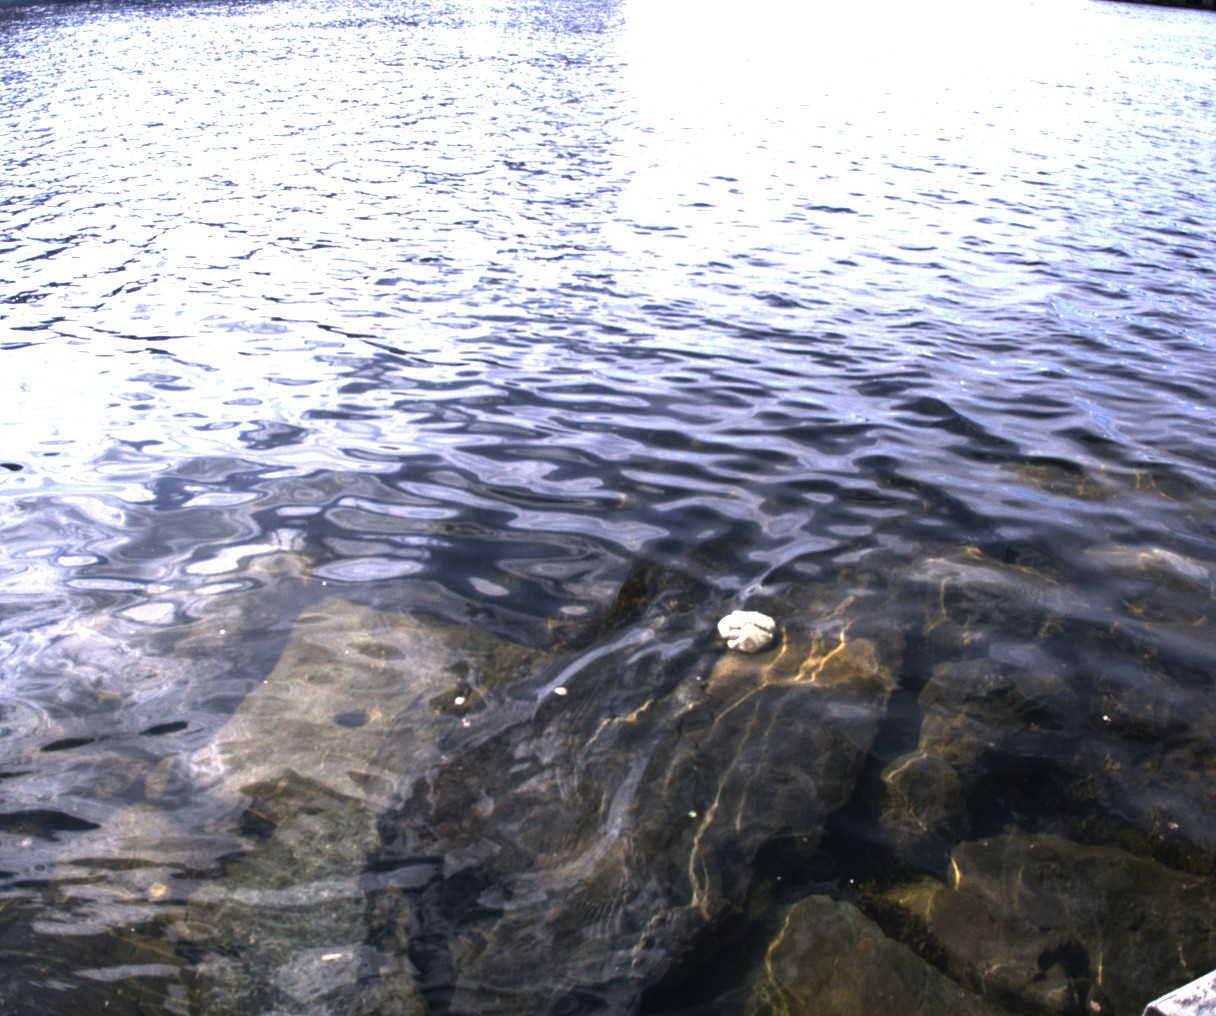
\includegraphics[width=\textwidth]{figures/pictures/img_4722_s0.jpg}
    \end{subfigure} \hfill
    \begin{subfigure}[T]{.49\textwidth}
        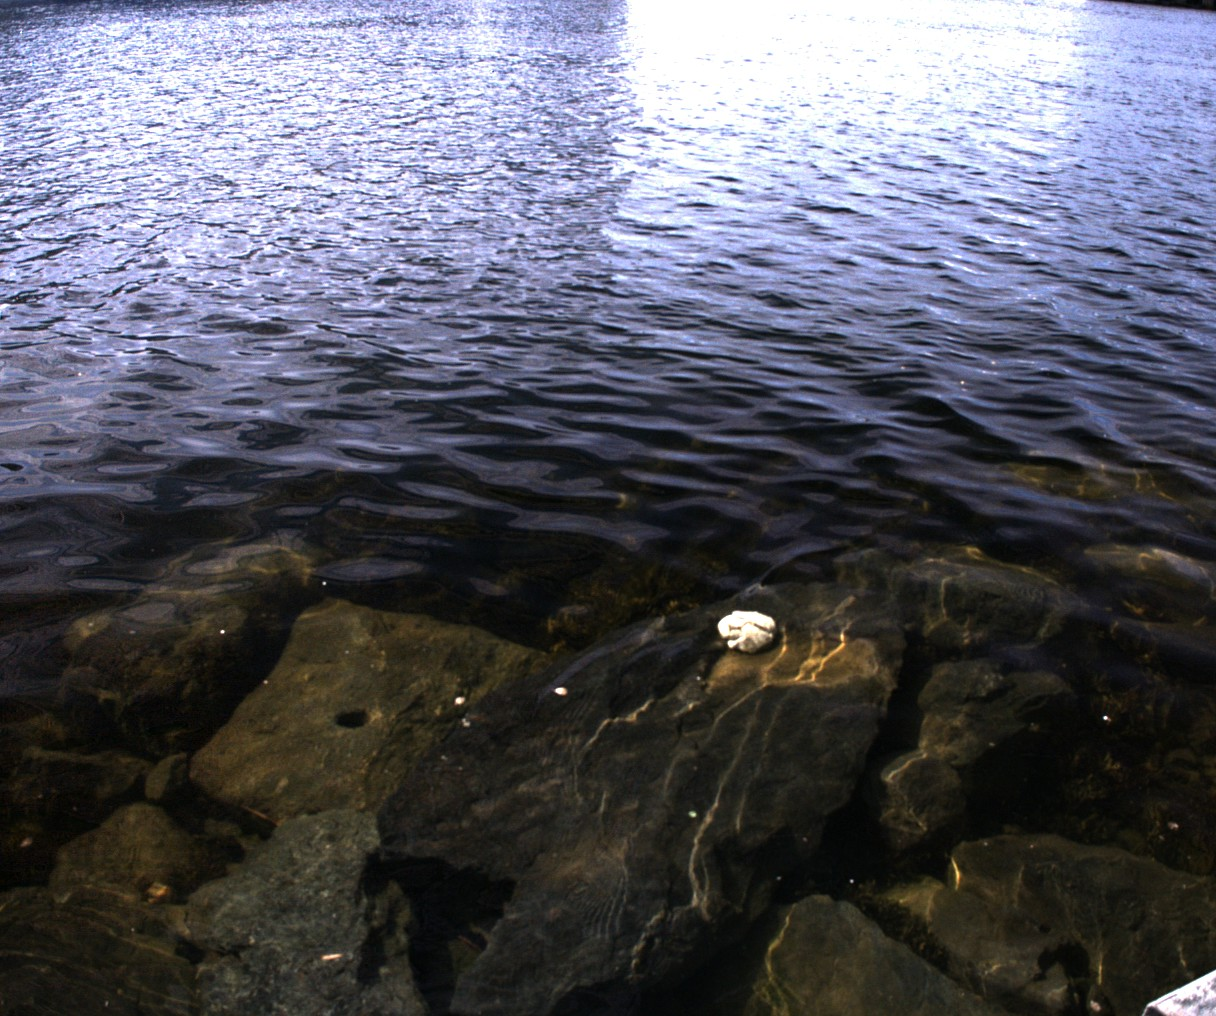
\includegraphics[width=\textwidth]{figures/pictures/img_4722_unpol.jpg}
    \end{subfigure}
    \caption{Image where the linearly polarized light is removed to see what's under the water surface. 
    Note that the degree of polarization follows the graph in Figure \ref{fig:dolp_graph}.}
\end{figure}
\vspace{-.5cm}

\begin{figure}[H]
    \begin{subfigure}[T]{.49\textwidth}
        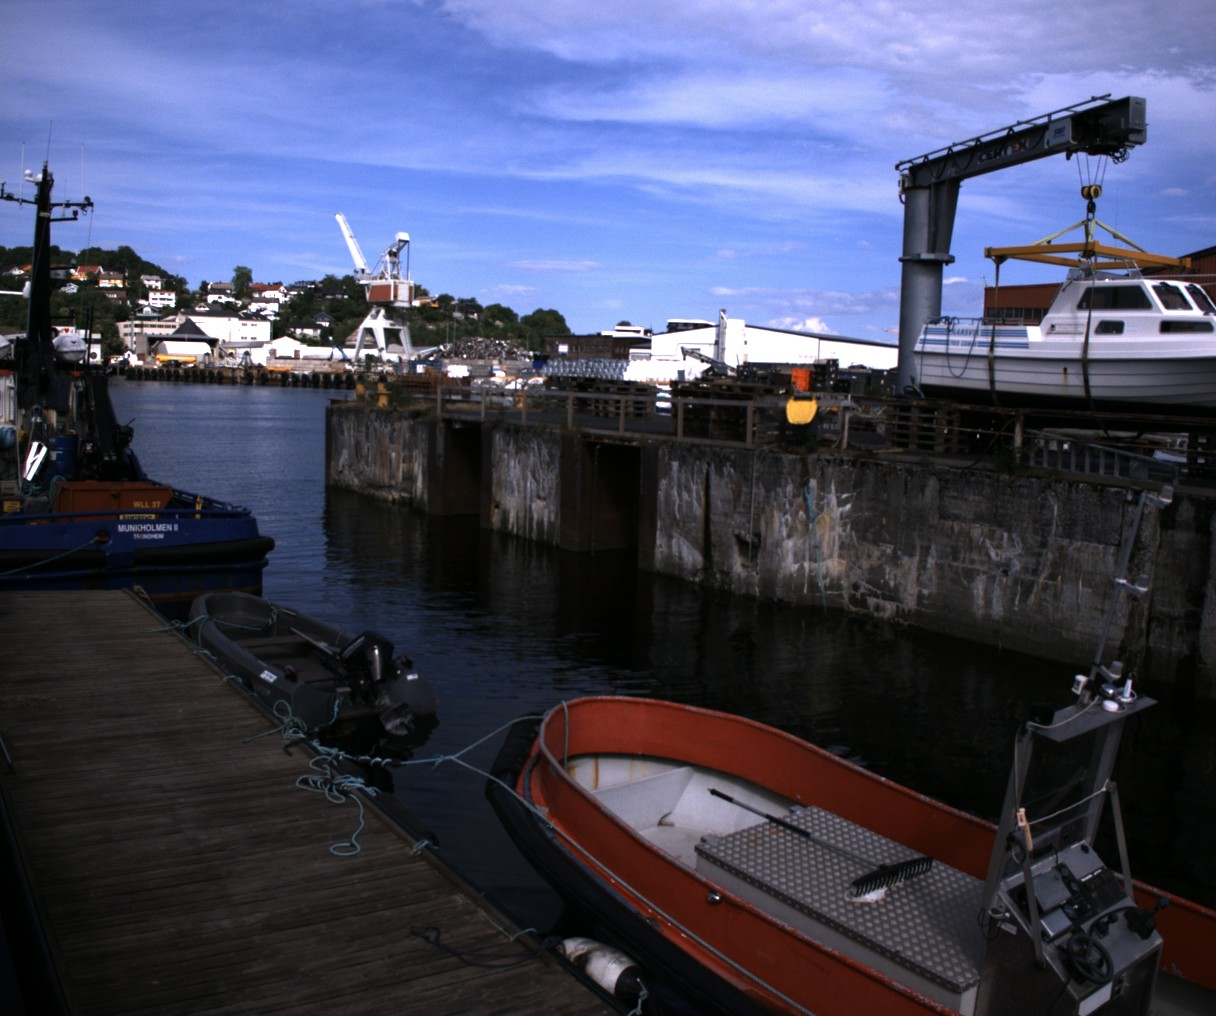
\includegraphics[width=\textwidth]{figures/pictures/img_2790_s0.jpg}
    \end{subfigure} \hfill
    \begin{subfigure}[T]{.49\textwidth}
        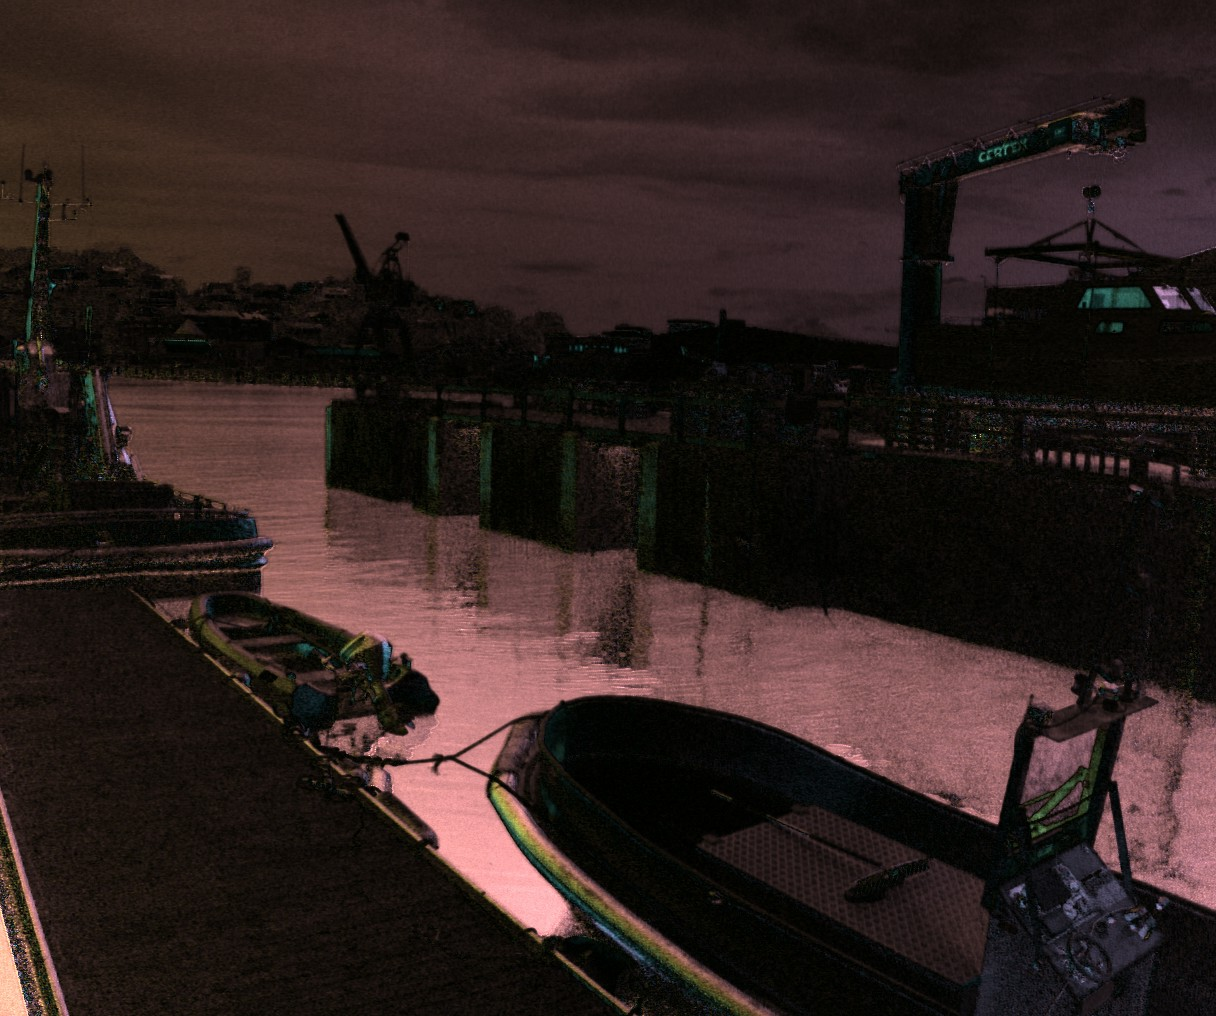
\includegraphics[width=\textwidth]{figures/pictures/img_2790_pol.jpg}
    \end{subfigure}
    \caption{Docking area demonstrating how the polarization of the water surface makes it more visible. 
    The visualization and color map are equivalent to Figure \ref{fig:cpfa_demosaicking}.}
\end{figure}
\vspace{-.7cm}

\begin{figure}[H]
    \begin{subfigure}[T]{.49\textwidth}
        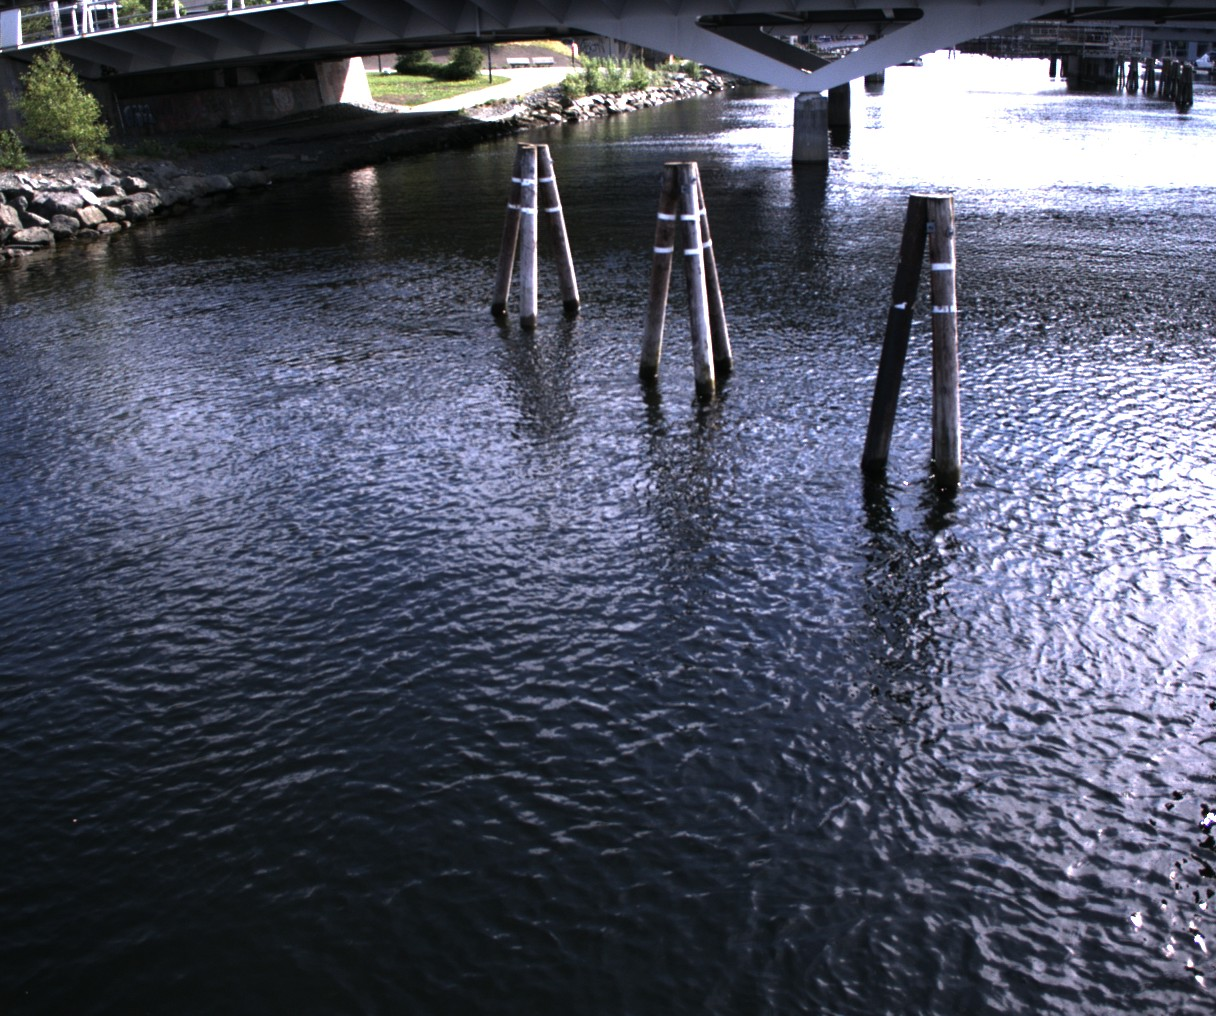
\includegraphics[width=\textwidth]{figures/pictures/img_7458_s0.jpg}
    \end{subfigure} \hfill
    \begin{subfigure}[T]{.49\textwidth}
        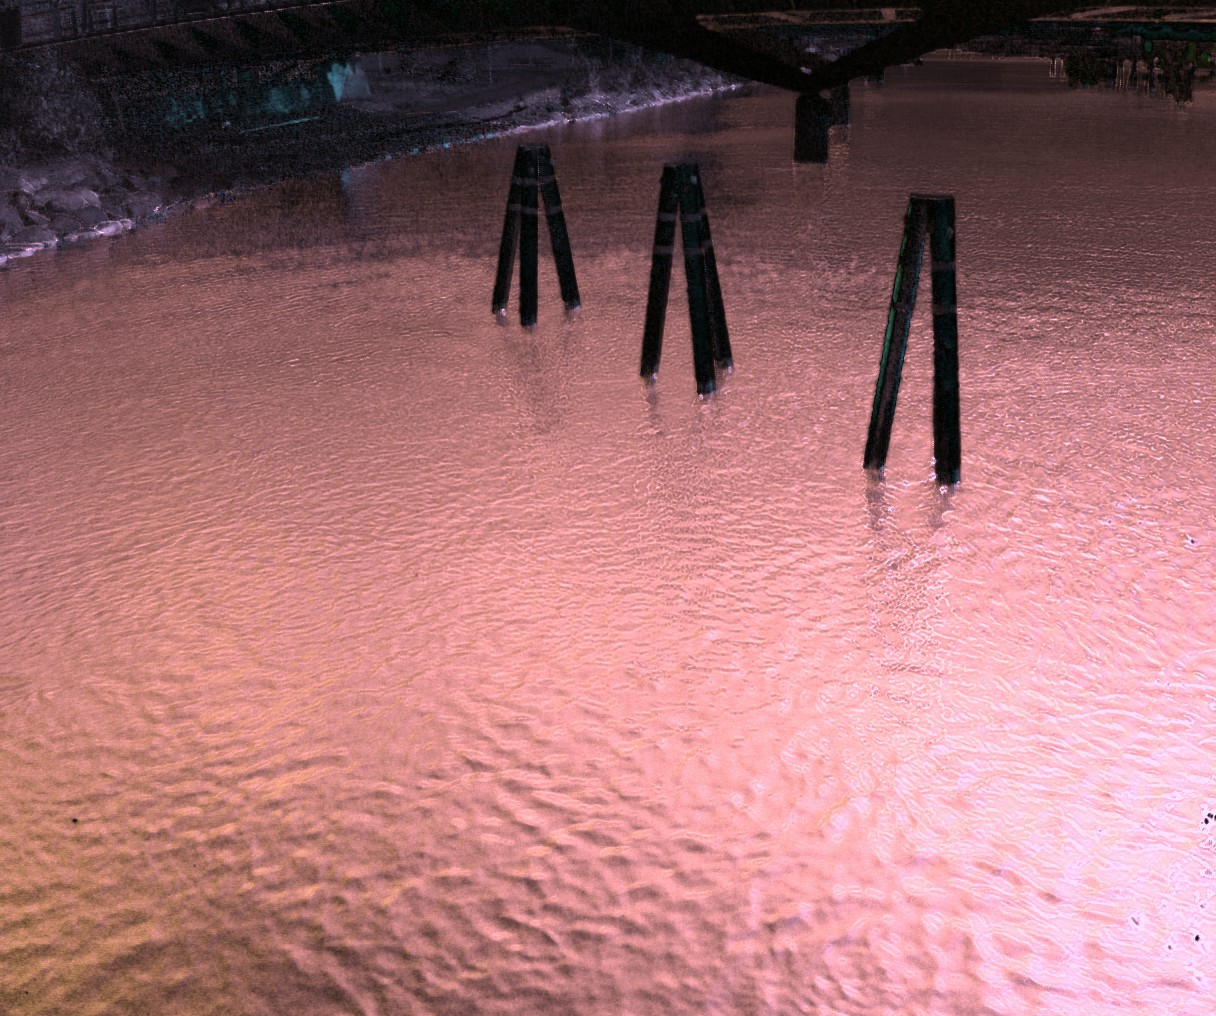
\includegraphics[width=\textwidth]{figures/pictures/img_7458_pol.jpg}
    \end{subfigure}
    \caption{Wooden posts protruding from the water.}
\end{figure}
\vspace{-.5cm}

\begin{figure}[H]
    \begin{subfigure}[T]{.49\textwidth}
        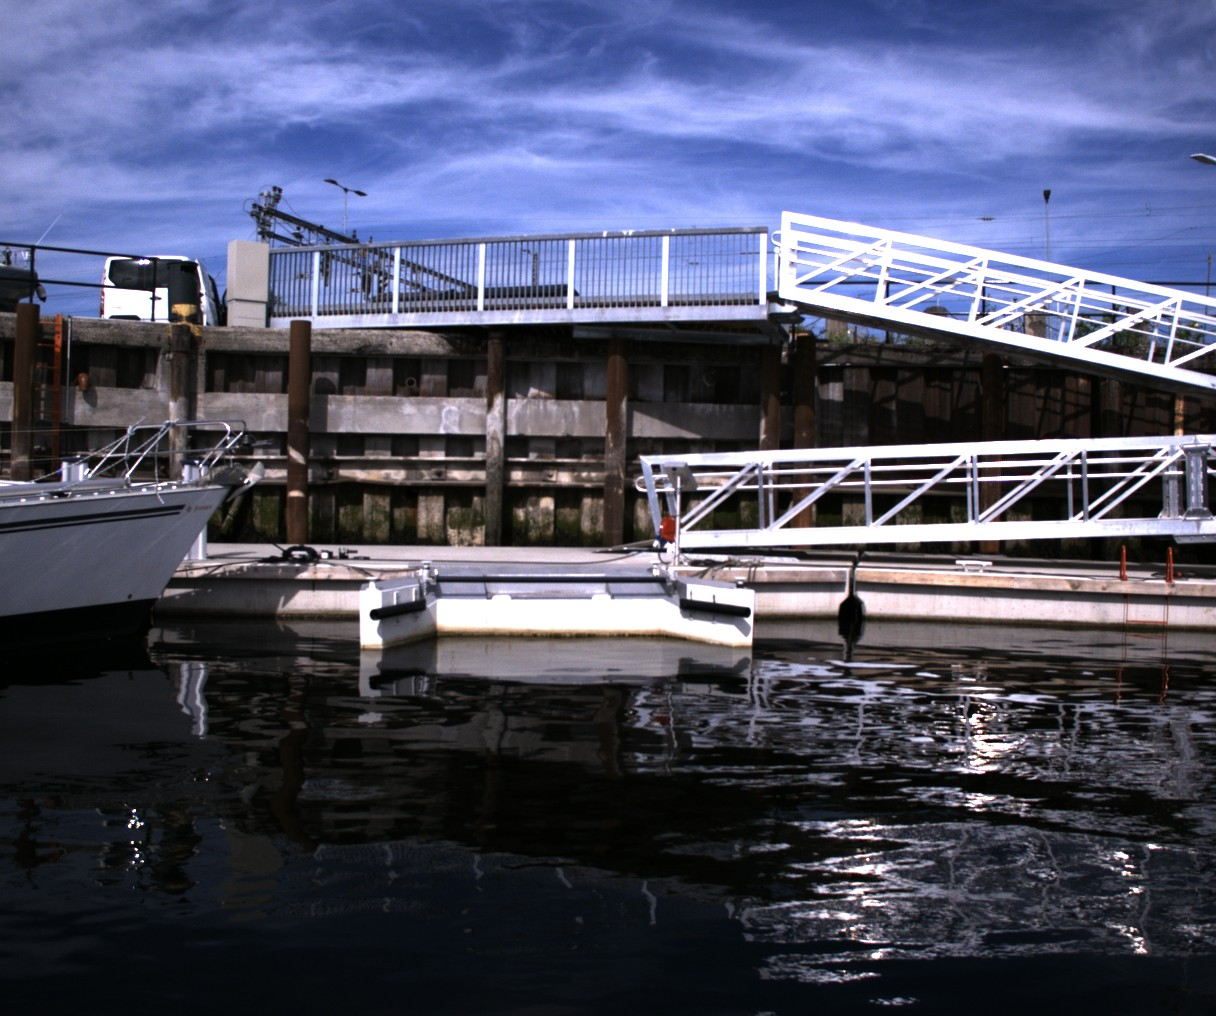
\includegraphics[width=\textwidth]{figures/pictures/img_11640_s0.jpg}
    \end{subfigure} \hfill
    \begin{subfigure}[T]{.49\textwidth}
        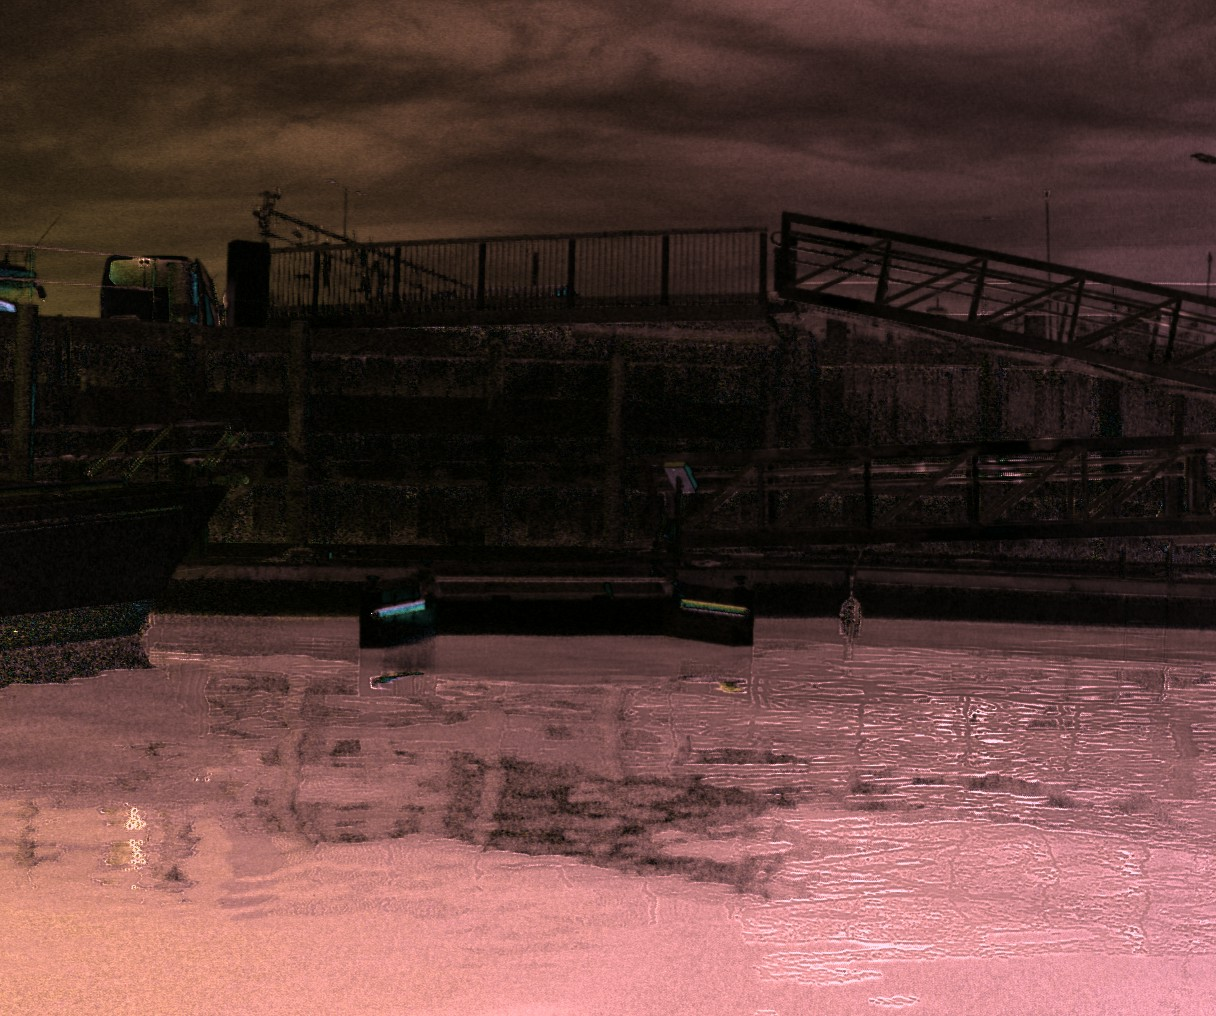
\includegraphics[width=\textwidth]{figures/pictures/img_11640_pol.jpg}
    \end{subfigure}
    \caption{Dock viewed from a vessel on the water.}
\end{figure}
\vspace{-.5cm}

\begin{figure}[H]
    \begin{subfigure}[T]{.49\textwidth}
        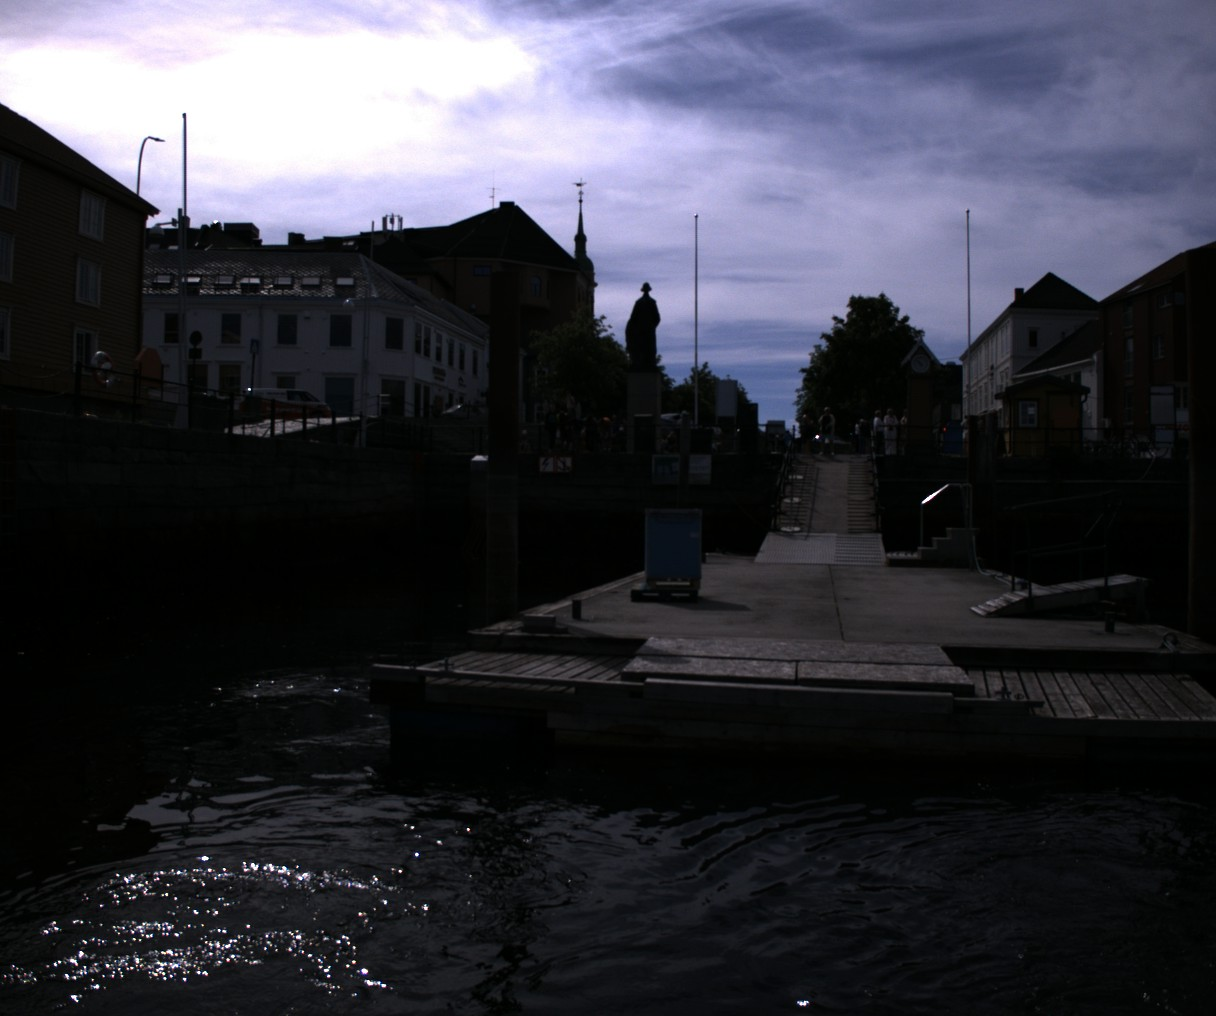
\includegraphics[width=\textwidth]{figures/pictures/img_10170_s0.jpg}
    \end{subfigure} \hfill
    \begin{subfigure}[T]{.49\textwidth}
        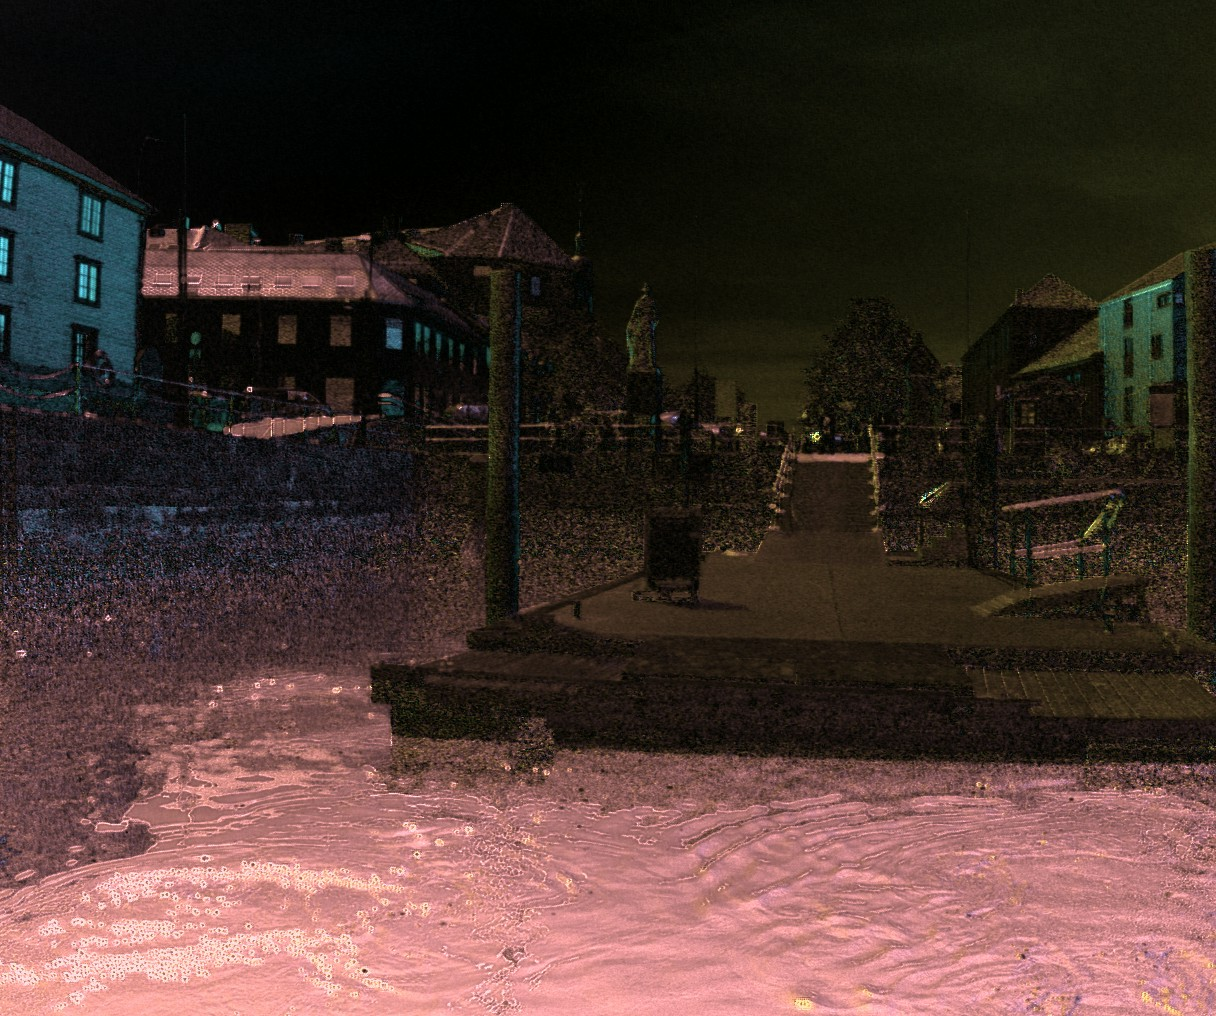
\includegraphics[width=\textwidth]{figures/pictures/img_10170_pol.jpg}
    \end{subfigure}
    \caption{Underexposed image of a dock viewed from the water.}
\end{figure}
\vspace{-.5cm}


\begin{figure}[H]
    \begin{subfigure}[T]{.49\textwidth}
        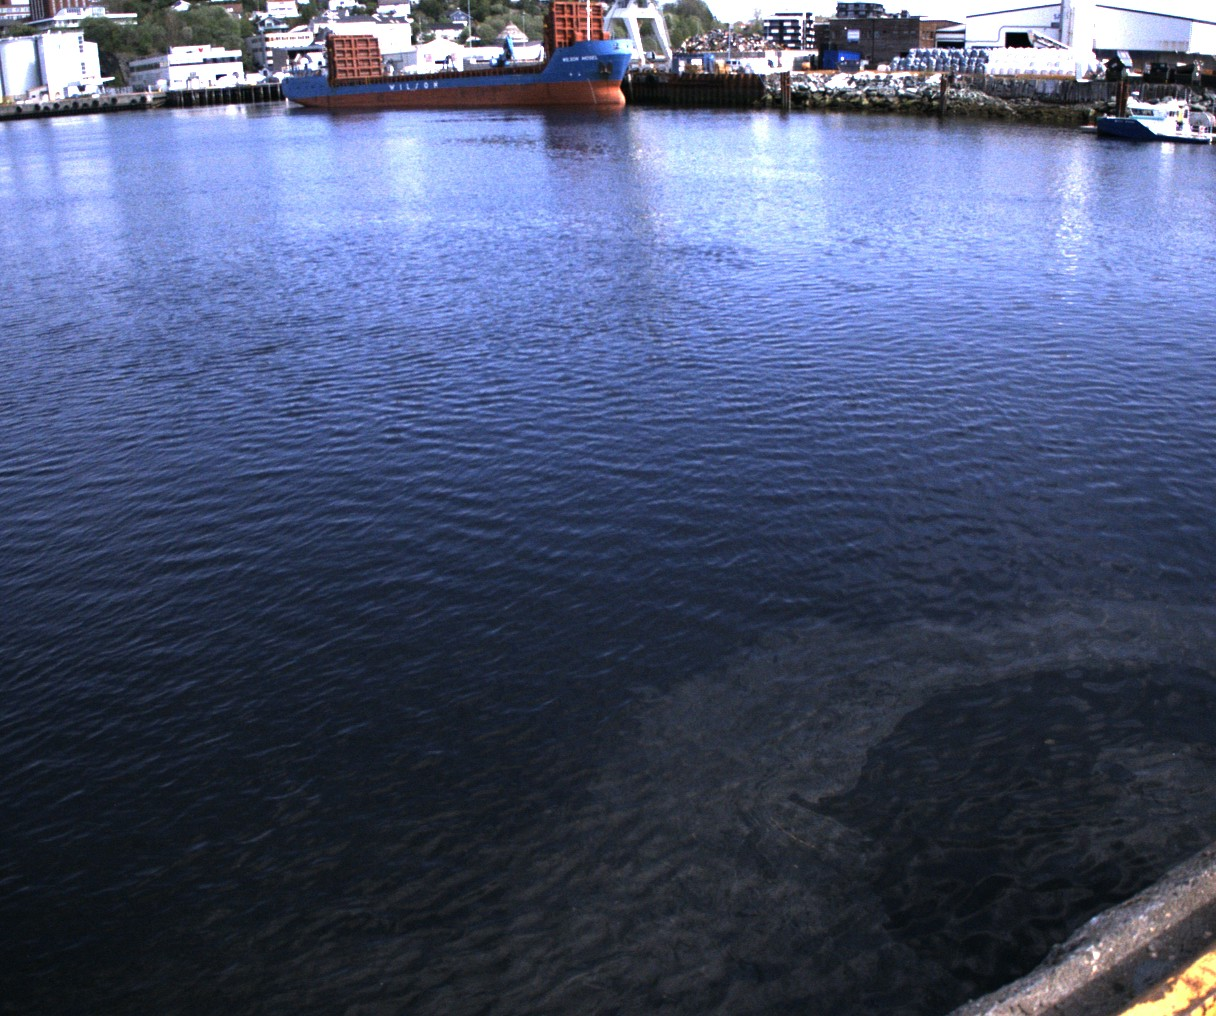
\includegraphics[width=\textwidth]{figures/pictures/img_3726_s0.jpg}
    \end{subfigure} \hfill
    \begin{subfigure}[T]{.49\textwidth}
        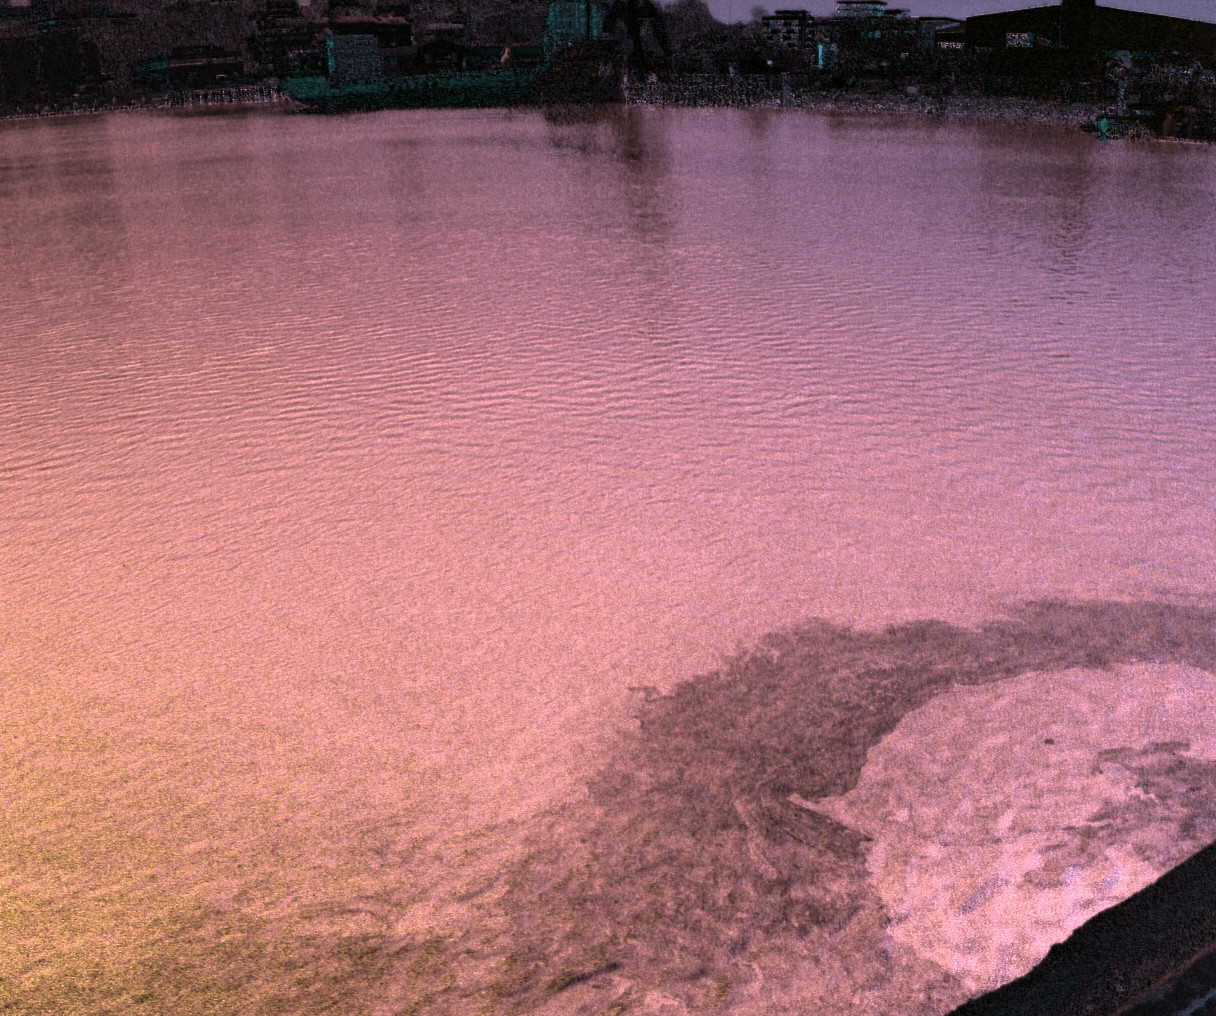
\includegraphics[width=\textwidth]{figures/pictures/img_3726_pol.jpg}
    \end{subfigure}
    \caption{Pollen on the water surface.}
\end{figure}
\vspace{-.5cm}

\begin{figure}[H]
    \begin{subfigure}[T]{.49\textwidth}
        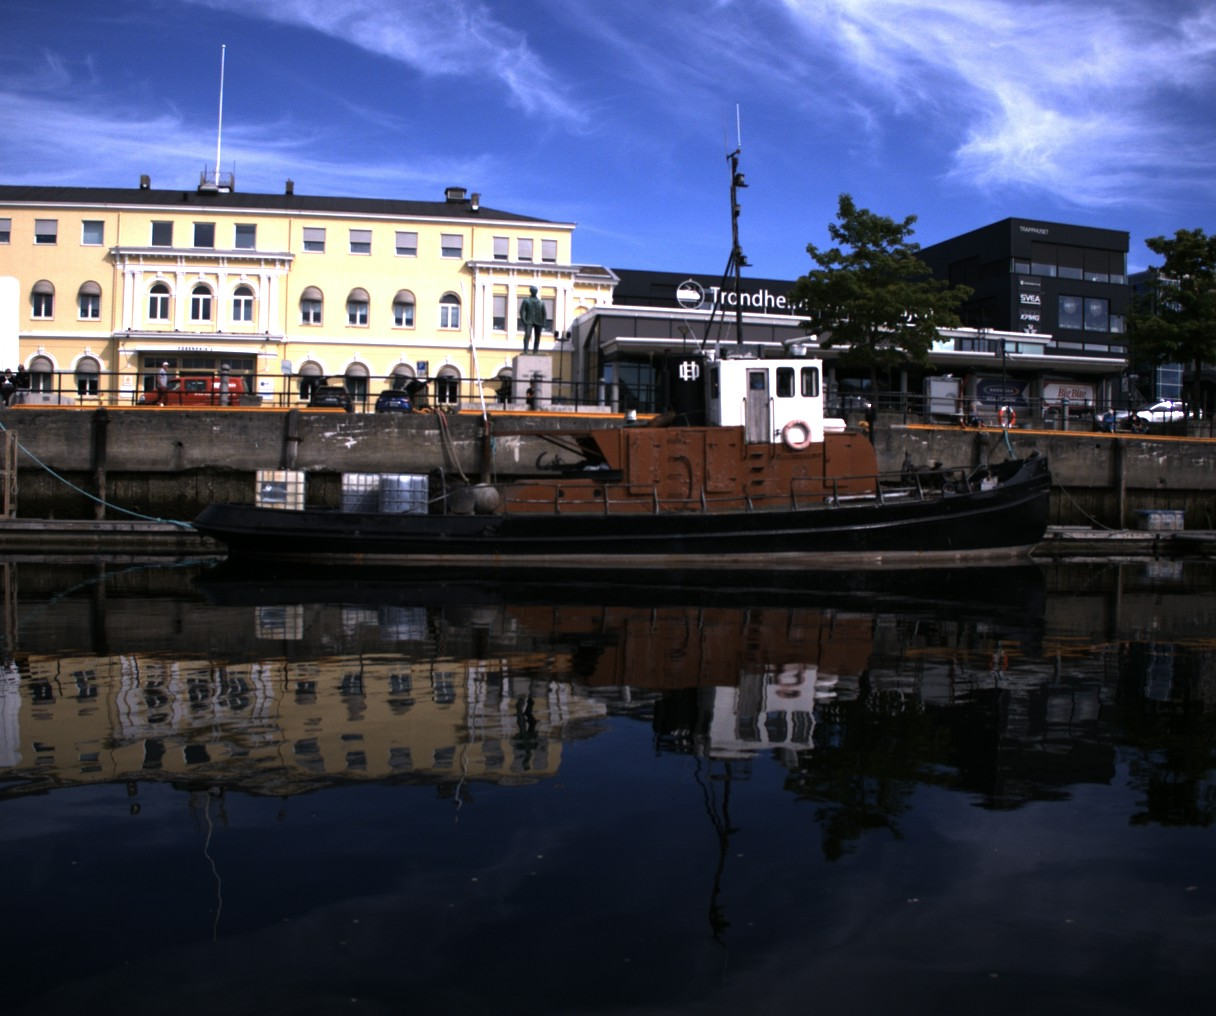
\includegraphics[width=\textwidth]{figures/pictures/img_4038_s0.jpg}
    \end{subfigure} \hfill
    \begin{subfigure}[T]{.49\textwidth}
        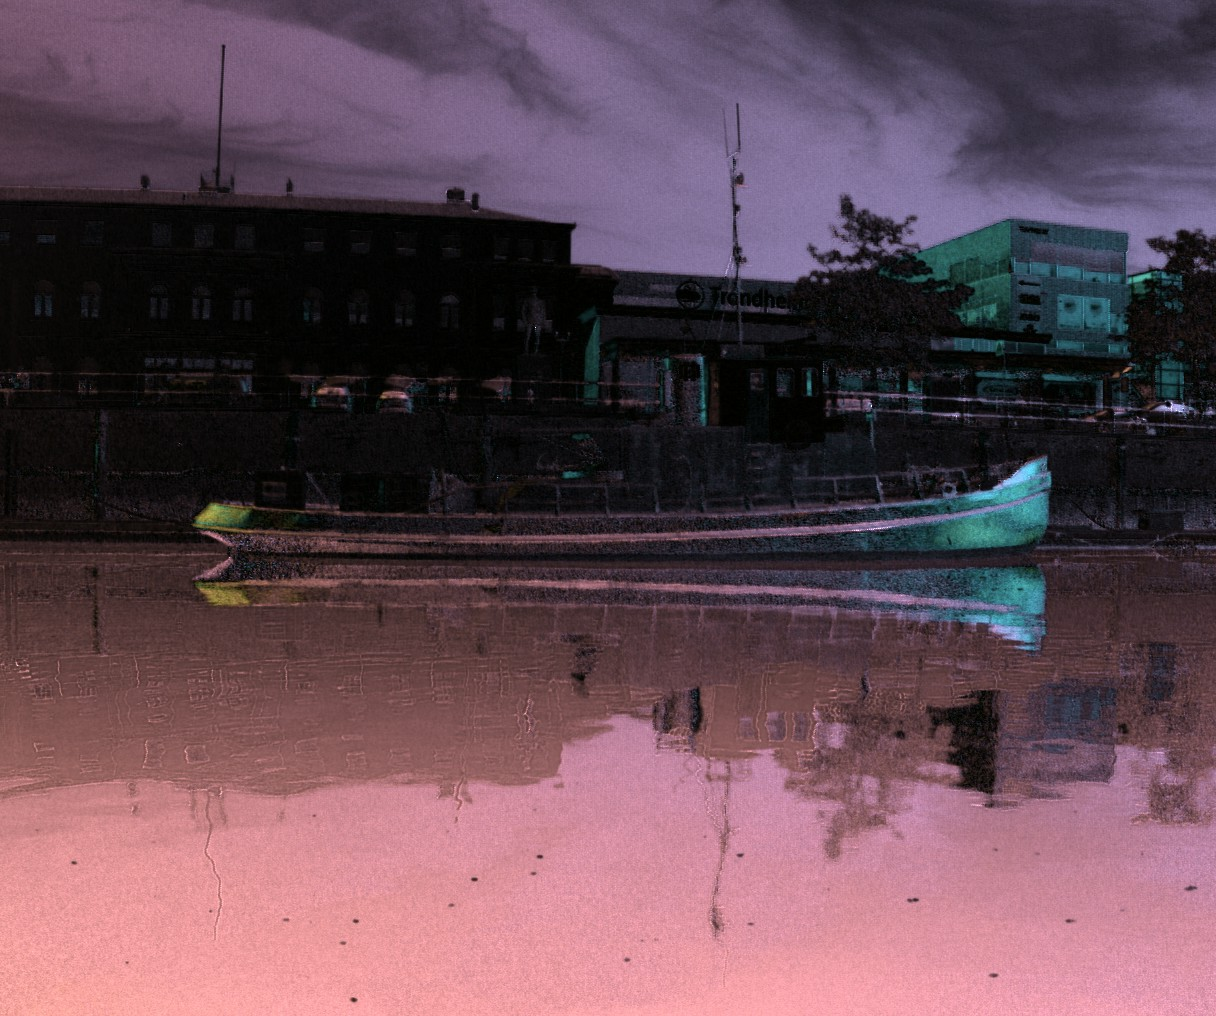
\includegraphics[width=\textwidth]{figures/pictures/img_4038_pol.jpg}
    \end{subfigure}
    \caption{A docked boat viewed from the water.}
\end{figure}
\vspace{-.5cm}

% \begin{figure}[H]
%     \begin{subfigure}[T]{.49\textwidth}
%         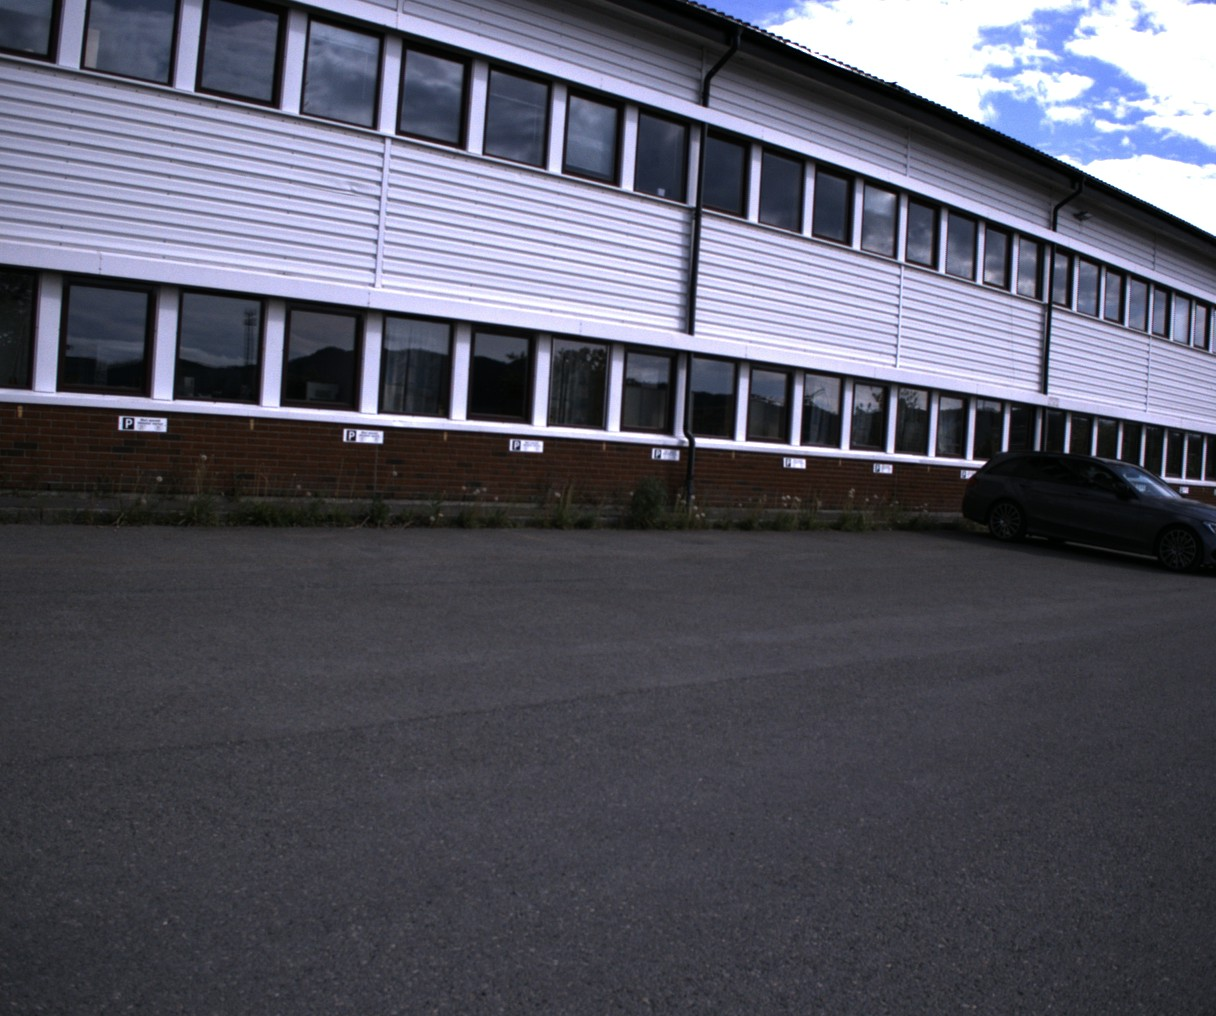
\includegraphics[width=\textwidth]{figures/pictures/img_5742_s0.jpg}
%     \end{subfigure} \hfill
%     \begin{subfigure}[T]{.49\textwidth}
%         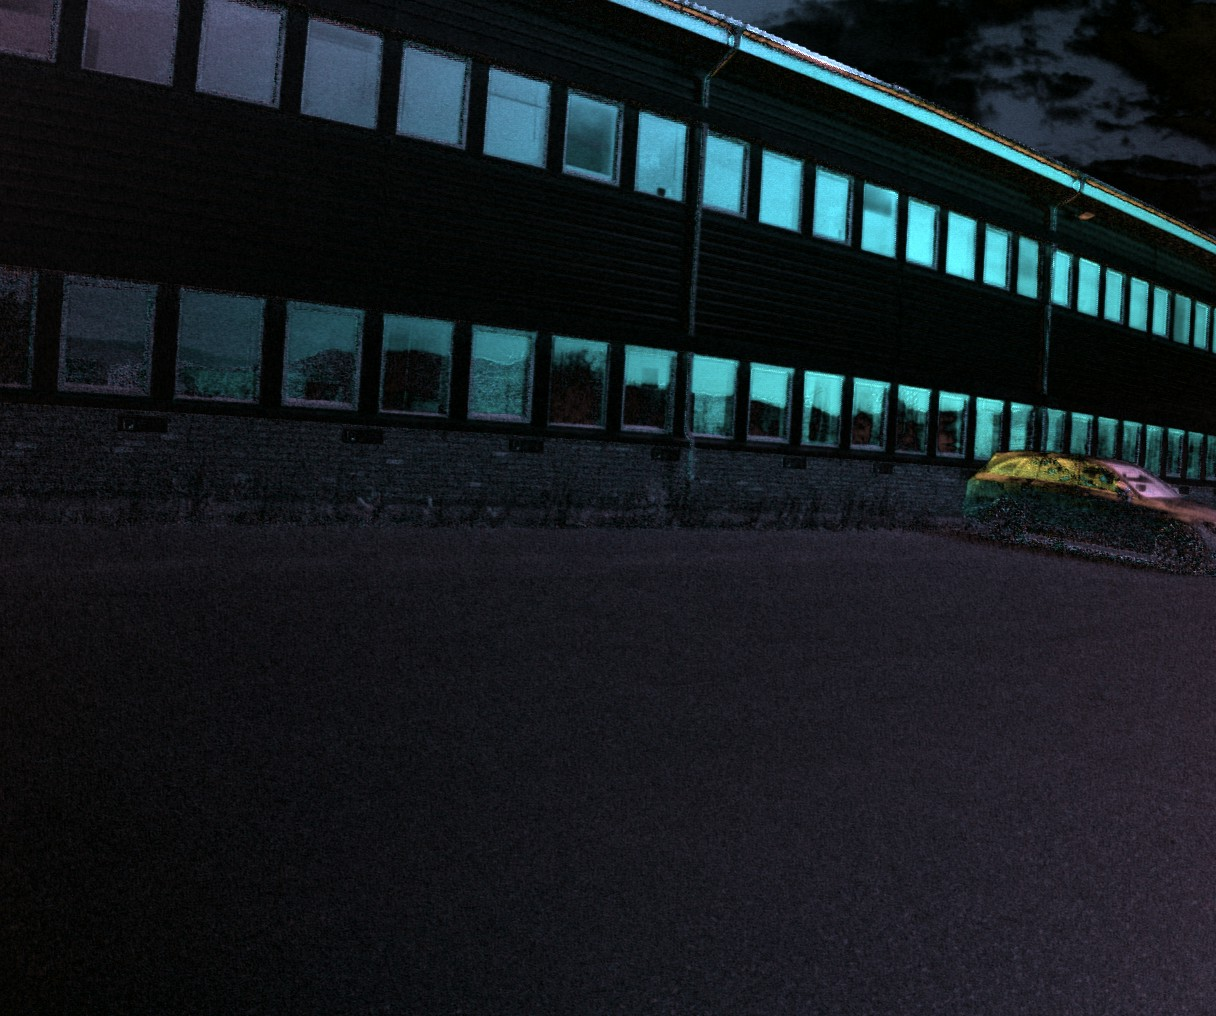
\includegraphics[width=\textwidth]{figures/pictures/img_5742_pol.jpg}
%     \end{subfigure}
%     \caption{Building with glass windows.}
% \end{figure}
% \vspace{-.5cm}
\begin{figure}[H]
    \begin{subfigure}[T]{.49\textwidth}
        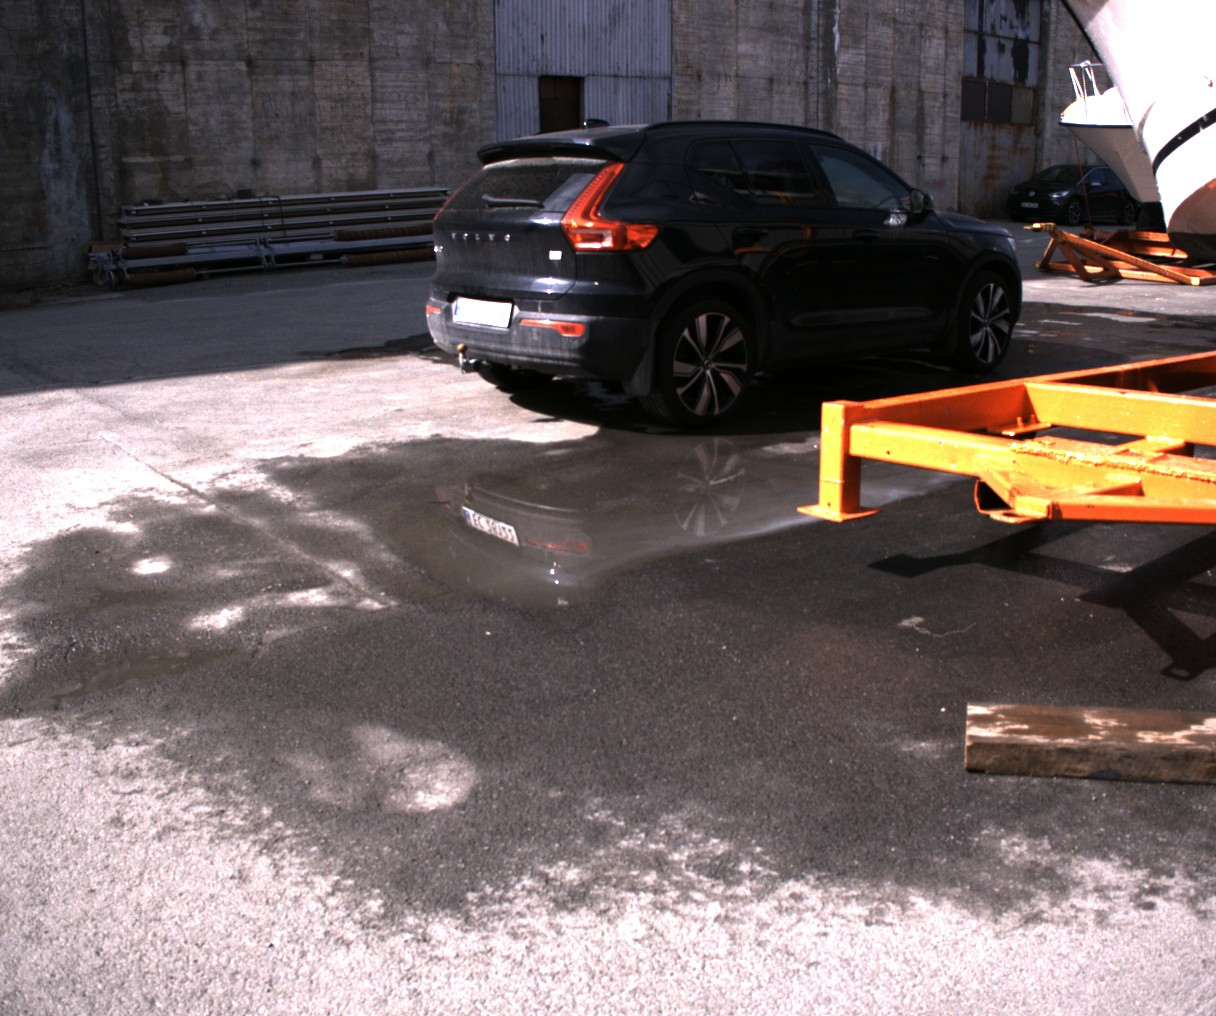
\includegraphics[width=\textwidth]{figures/pictures/img_1116_s0.jpg}
    \end{subfigure} \hfill
    \begin{subfigure}[T]{.49\textwidth}
        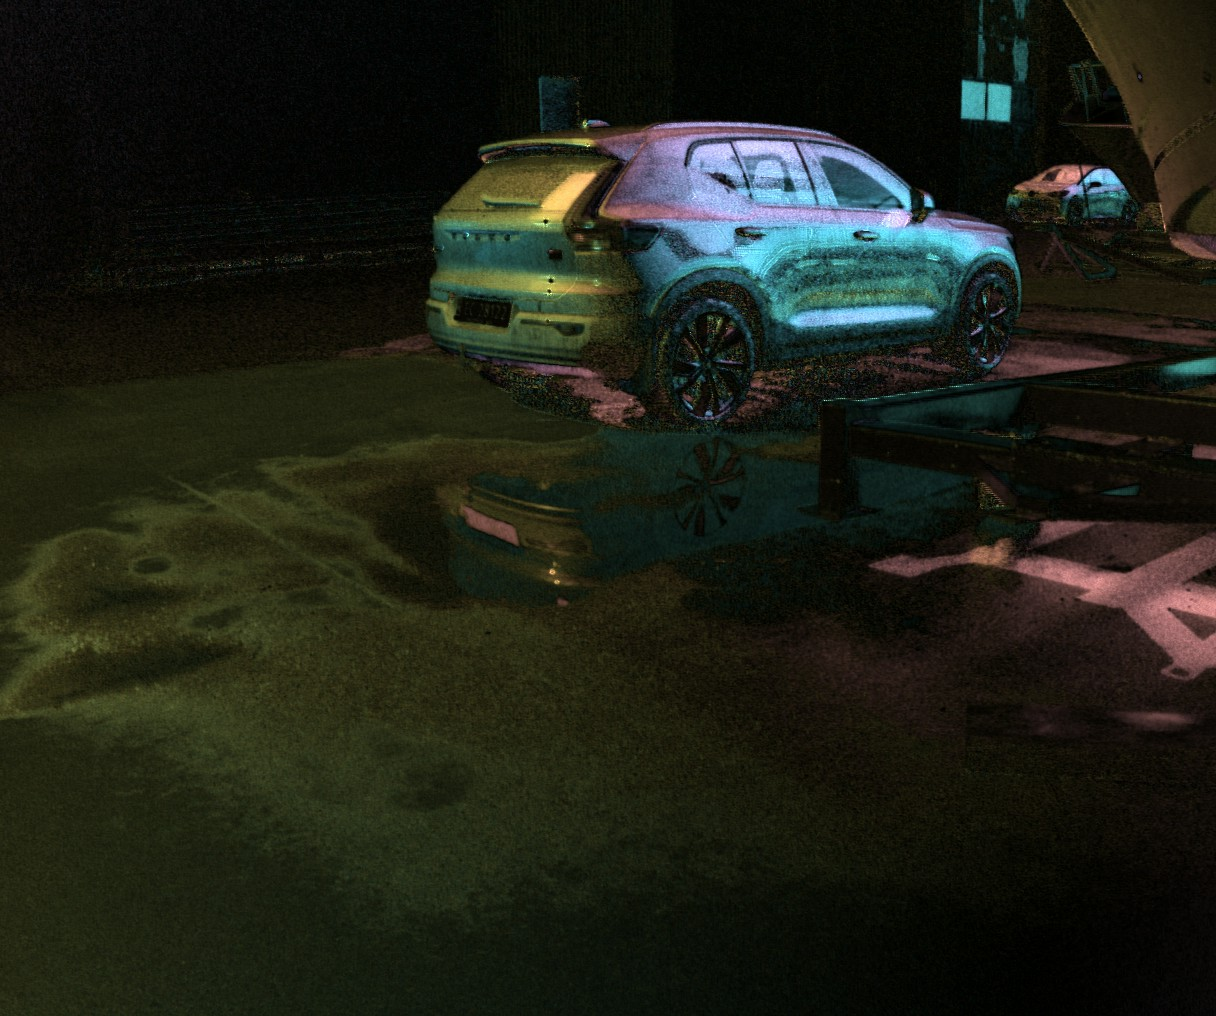
\includegraphics[width=\textwidth]{figures/pictures/img_1116_pol.jpg}
    \end{subfigure}
    \caption{A black car.}
\end{figure}
\vspace{-.5cm}


\begin{figure}[H]
    \begin{subfigure}[T]{.49\textwidth}
        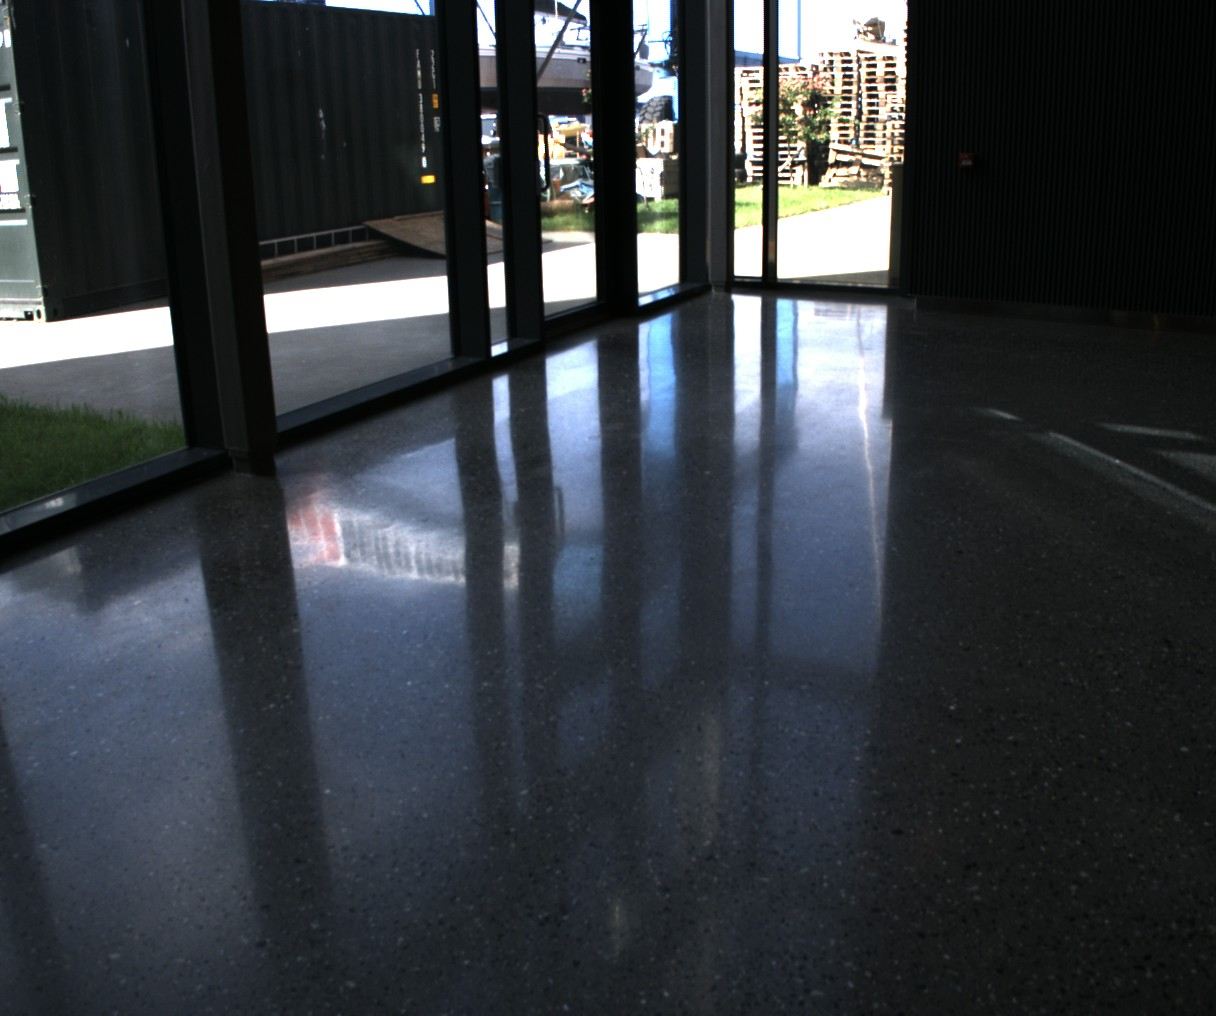
\includegraphics[width=\textwidth]{figures/pictures/img_9222_s0.jpg}
    \end{subfigure} \hfill
    \begin{subfigure}[T]{.49\textwidth}
        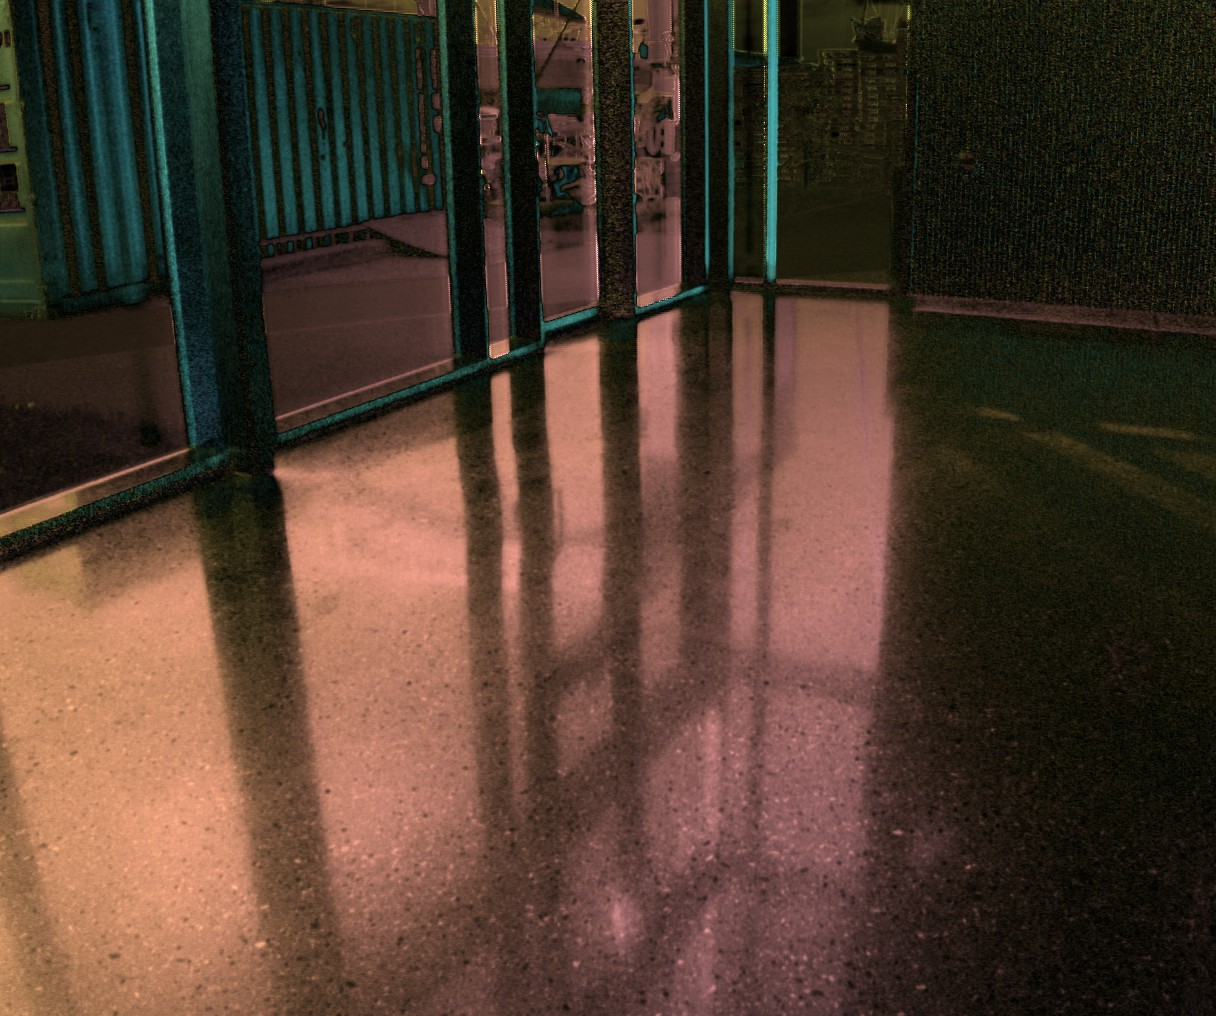
\includegraphics[width=\textwidth]{figures/pictures/img_9222_pol.jpg}
    \end{subfigure}
    \caption{Stone floor with reflections.}
\end{figure}
\vspace{-.5cm}

 \begin{figure}[H]
     \begin{subfigure}[T]{.49\textwidth}
         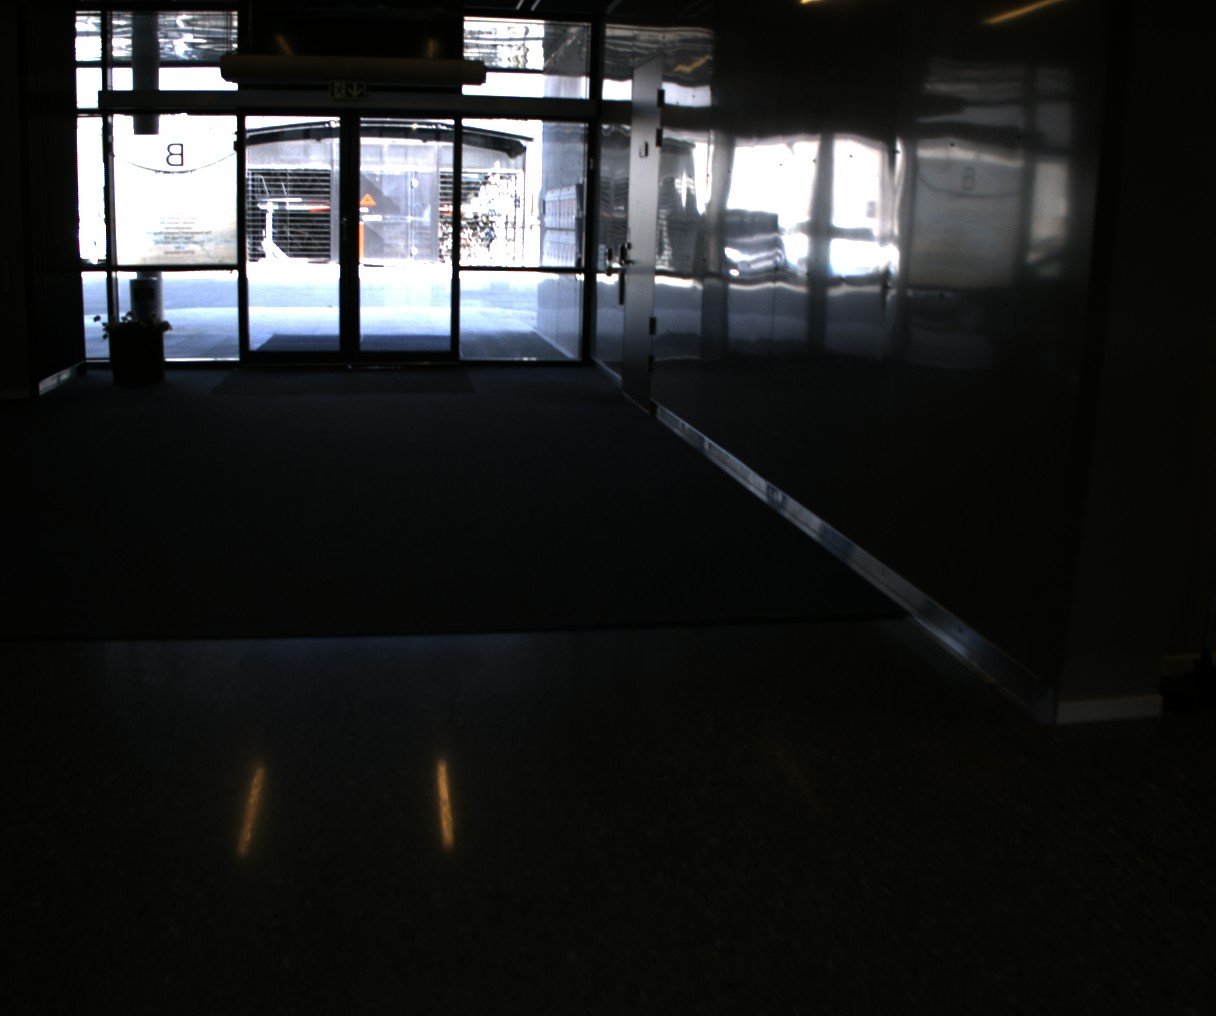
\includegraphics[width=\textwidth]{figures/pictures/img_9306_s0.jpg}
     \end{subfigure} \hfill
    \begin{subfigure}[T]{.49\textwidth}
         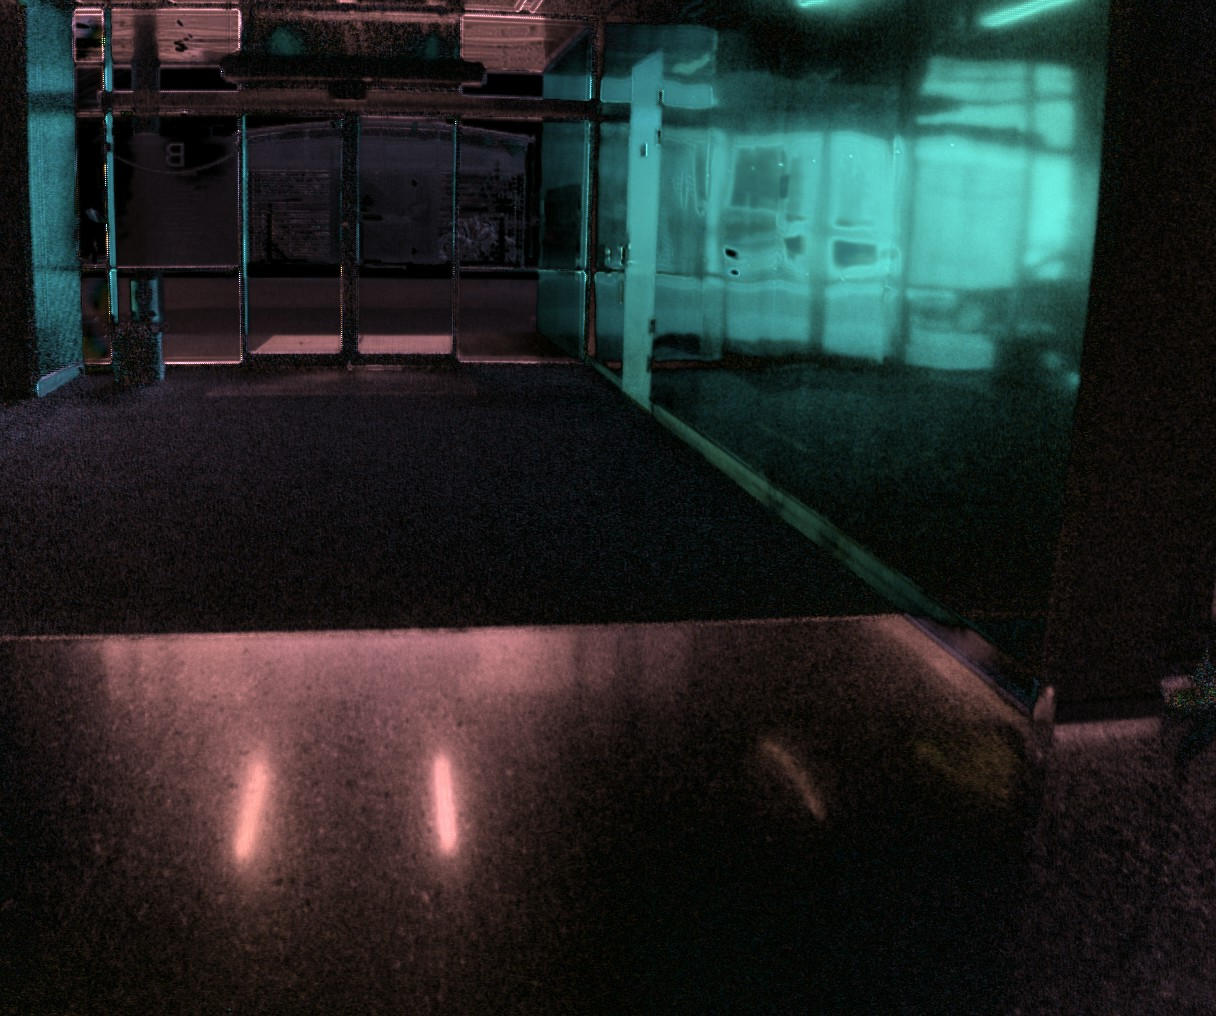
\includegraphics[width=\textwidth]{figures/pictures/img_9306_pol.jpg}
     \end{subfigure}
     \caption{High contrast indoor environment.}
 \end{figure}
 \vspace{-.5cm}



